% Compilação: pdflatex Relatorio_STR_M3.tex (duas vezes).
% Requer: IEEEtran, pgfplots (TeX Live completo).
% Dados: resultados/etapa1_teste.md ... etapa4_teste.md, analise_experimento_B.md,
%        analise_experimento_C.md e resultado_exp_d.md.
\documentclass[conference,a4paper]{IEEEtran}
\usepackage[utf8]{inputenc}
\usepackage[T1]{fontenc}
\usepackage{amsmath,amssymb}
\usepackage{booktabs,array}
\usepackage{graphicx,microtype}
\usepackage{pgfplots}
\pgfplotsset{compat=1.16}
\usepackage[hidelinks]{hyperref}
\renewcommand{\abstractname}{Resumo}
\renewcommand{\IEEEkeywordsname}{Palavras-chave}
\renewcommand{\refname}{Referências}
\renewcommand{\tablename}{Tabela}
\renewcommand{\figurename}{Figura}
\hyphenation{FreeRTOS}

\title{Medição do tempo de resposta e estimativa de WCRT da codificação de Huffman em ESP32 com FreeRTOS em quatro escopos de teste}
% PREENCHER: nomes e RAs dos integrantes (grupo de até 2 alunos).
\author{\IEEEauthorblockN{[Nome do integrante 1] (RA [RA 1]) e [Nome do integrante 2] (RA [RA 2])}
\IEEEauthorblockA{Engenharia de Computação --- Universidade do Vale do Itajaí (UNIVALI)\\Sistemas em Tempo Real --- Atividade M3\\Professores: Michael Douglas C A e Felipe Viel}}

\begin{document}
\maketitle

\begin{abstract}
Este trabalho mede o tempo de resposta da codificação de Huffman em uma ESP32 com FreeRTOS, em quatro escopos de teste com estresse crescente: tarefa, comportamental, intertarefas e sistema. O deadline foi fixado uma única vez, a partir da etapa 1, em $D = 13519\ \mu$s. O HWM subiu de 11266 $\mu$s (tarefa isolada) para 13498 $\mu$s (sistema), cerca de 20\%, com a mesma lógica de codificação. Em rodadas de 10\,000 ativações do sistema, o HWM ainda subiu depois de 1\,000 amostras em duas de três rodadas. Uma margem de 10\% sobre o HWM da etapa 1 não cobre o sistema; a de 25\% cobre, com folga de 585 $\mu$s. Variando $D$ sobre as mesmas medições, o sistema passou de 15\% de ativações no prazo ($D = 11266\ \mu$s) a 100\% ($D \geq 13500\ \mu$s), e o modelo (m,k)-firme descreveu a faixa intermediária, por exemplo (16,20)-firme em $D = 12393\ \mu$s.
\end{abstract}

\begin{IEEEkeywords}
FreeRTOS, ESP32, tempo real, WCRT, HWM, (m,k)-firme.
\end{IEEEkeywords}

\section{Introdução}
Em muitos sistemas de tempo real, a análise rigorosa do tempo de resposta é inviável, e o tempo de resposta precisa ser medido. O pior caso (WCRT) ocorre com pouca frequência, e as condições que o provocam costumam ser desconhecidas. O maior tempo observado, o HWM (\emph{High Water Mark}), é uma aproximação otimista do WCRT, e a margem de segurança aplicada sobre ele depende da variabilidade das medições. Quando o WCRT não é alcançável, a tolerância a perdas de deadline pode ser especificada pelo percentual de deadlines cumpridos, pelo \emph{skip factor} e pelo modelo (m,k)-firme.

O objetivo é medir a mesma tarefa, a codificação de Huffman sobre um array aleatório de caracteres, em quatro escopos com estresse crescente, e responder, com dados, à questão: \emph{se a cobertura de código chega a 100\%, por que o HWM continua crescente? E, quando o WCRT não é alcançável, como o modelo (m,k)-firme transforma as medições em um critério testável?} Todas as medições foram feitas em uma ESP32 física.

A Seção II descreve a plataforma e a tarefa. A Seção III apresenta a metodologia e a definição do deadline. A Seção IV traz os resultados por etapa, e as Seções V a VII, os experimentos B, C e D. A Seção VIII trata do (m,k)-firme e de seus limites. As Seções IX e X trazem as ameaças à validade e a conclusão.

\section{Plataforma e tarefa sob teste}
\subsection{Plataforma}
A Tabela I resume a plataforma. Em todas as rodadas, a saída completa do monitor foi guardada.

\begin{table}[!t]
\centering
\caption{Plataforma de medição.}
\small
\setlength{\tabcolsep}{3pt}
\begin{tabular}{p{2.4cm}p{5.6cm}}
\toprule
Item & Valor \\
\midrule
Placa & ESP32 (modelo 1), revisão v3.1, 2 núcleos \\
CPU & 240 MHz fixos; \emph{power management} desligado (equivale ao governor) \\
SO / RTOS & FreeRTOS (ESP-IDF v6.1), tick de 10 ms \\
Otimização & \texttt{-O2} \\
Wi-Fi & Componente compilado; não iniciado pelo programa \\
Medição & \texttt{clock\_gettime(CLOCK\_MONOTONIC)}, resolução em $\mu$s \\
Tarefas do FreeRTOS & 6 (etapas 1 e 3) e 7 (etapa 4), contando as do ESP-IDF \\
Watchdog de tarefas & Desligado nas rodadas de sistema (etapa 4 e experimentos B e D) \\
\bottomrule
\end{tabular}
\end{table}

\subsection{Tarefa e validação}
A tarefa sob teste constrói a árvore de Huffman, gera os códigos, codifica e decodifica um texto aleatório de 1\,000 caracteres, com valores de 1 a 255, gerados por xorshift32. A semente base é 12345; nas etapas 1 e 2, a semente de cada ativação é 12345 + $i$, e nas etapas 3 e 4, o sensor usa a semente 12345. Cada ativação decodifica e compara com a entrada (\texttt{strcmp}). O critério de aprovação é zero erros: todas as rodadas apresentaram zero erros. A geração da entrada e a liberação de memória ficam fora do tempo medido. A tarefa é implementada em C, em um único cabeçalho (\texttt{huffman.h}), e todas as estatísticas são calculadas pelo firmware depois da medição, sem impressão durante a coleta.

\section{Metodologia}
\subsection{Etapas, casos de teste e procedimento}
A Tabela II descreve as quatro etapas. Em todas, a tarefa medida é a mesma.

\begin{table*}[!t]
\centering
\caption{Etapas do experimento. Todas medem a mesma tarefa de Huffman (1\,000 caracteres).}
\small
\setlength{\tabcolsep}{3pt}
\begin{tabular}{llp{9.4cm}rr}
\toprule
Etapa & Escopo & Caso de teste e estresse & $N$ & Rodadas \\
\midrule
1 & Tarefa & Huffman isolada, com validação. Pausa de um tick fora da medição entre ativações & 1\,000 & 3 \\
2 & Comportamental & Um evento por vez: um \emph{timer} \emph{one-shot} de 20 ms, armado a cada ativação, libera a tarefa por semáforo (interrupção simulada) & 1\,000 & 3 \\
3 & Intertarefas & Sensor (prioridade 6, 10 ms) escreve um texto novo no buffer compartilhado; Huffman (prioridade 5, 30 ms) copia o buffer sob mutex e codifica. A cópia entra na medição & 1\,000 & 3 \\
4 & Sistema & Etapa 3 mais: evento a cada 20 ms (prioridade 4) com uma Huffman por evento, não medida; carga de CPU (prioridade 1, fixada no core 0), 3 ms ocupada e 3 ms livre, cerca de 50\% do core & 1\,000 e 10\,000 & 3 e 3 \\
\bottomrule
\end{tabular}
\end{table*}

\subsection{Descrição de cada etapa}
Em todas as etapas, as entradas são: $N$ ativações, texto de 1\,000 caracteres e semente 12345. O comportamento esperado é a decodificação reproduzir exatamente o texto de entrada, em todas as ativações.

\emph{Etapa 1 (tarefa).} Uma única tarefa (prioridade 5, sem core fixo) executa $N$ ativações em sequência: gera o texto, executa a Huffman (árvore, códigos, codificação, decodificação), valida e registra o tempo de cada ativação e de cada passo interno. Entre ativações, a tarefa bloqueia por um tick, fora da medição, para a tarefa \texttt{IDLE} rodar. Não há estresse. O D é definido a partir do HWM desta etapa.

\emph{Etapa 2 (comportamental).} A tarefa responde a um evento externo por vez. A cada ativação, a própria tarefa arma um \emph{timer} \emph{one-shot} de 20 ms e espera em um semáforo; quando o \emph{timer} dispara, ele guarda o instante do evento e libera a tarefa. A resposta é medida do disparo ao fim da Huffman. É uma interrupção simulada: há um único evento pendente de cada vez.

\emph{Etapa 3 (intertarefas).} Duas tarefas periódicas, com taxas diferentes, compartilham um buffer protegido por mutex. O sensor (prioridade 6) escreve um texto novo a cada 10 ms. A Huffman (prioridade 5), a cada 30 ms, copia o buffer sob o mutex e codifica. A medição vai do fim do atraso periódico ao fim da Huffman, e inclui a cópia. O estresse é a contenção pelo mutex, o bloqueio e a preempção do sensor sobre a Huffman.

\emph{Etapa 4 (sistema).} Junta a etapa 3 com duas outras fontes de concorrência: um evento a cada 20 ms que dispara uma Huffman em uma tarefa de prioridade 4 (não medida, só ocupa a CPU) e uma tarefa de carga de prioridade 1, fixada no core 0, que fica 3 ms ocupada e 3 ms livre (cerca de 50\% do core). A Huffman periódica continua sendo a única tarefa medida.

\emph{Procedimento e critério.} Cada etapa foi executada em três rodadas, com a placa reiniciada entre elas, e a saída completa do monitor foi guardada. Uma etapa é aprovada se todas as ativações têm validação correta (zero erros), se há pelo menos 1\,000 ativações e se as condições do teste foram registradas. Como o objetivo em tempo real é buscar o pior caso, o estresse cresce de uma etapa para a seguinte, na tentativa de fazer o sistema perder o prazo.

O estresse da etapa 4 foi escolhido para disputar a CPU e o buffer com a tarefa medida: a Huffman por evento ocupa o processador em paralelo com a Huffman periódica, e a carga simula outra atividade do sistema. As tarefas de Huffman não têm core fixo, então podem compartilhar o core 0 com a carga.

O procedimento de cada etapa foi: compilar e gravar com \texttt{idf.py build flash monitor}, deixar a rodada terminar, copiar a saída do monitor, reiniciar a placa e repetir. O critério de aprovação foi zero erros, pelo menos 1\,000 ativações por cenário, 10\,000 ativações para a convergência (experimento B) e condições do teste registradas a cada rodada. As periodicidades usam \texttt{vTaskDelay}, então o período real é um pouco maior que o nominal: cerca de 30 ms mais o tempo de resposta (cerca de 42 ms por ciclo na etapa 4).

\subsection{Resposta e deadline}
O tempo de resposta da etapa 1 é o tempo de execução da Huffman. Nas etapas 2 a 4, é medido do instante de liberação (disparo do \emph{timer} ou fim do \texttt{vTaskDelay}) até o fim da codificação. Uma ativação perde o deadline se a resposta ultrapassa $D$.

O deadline foi definido uma única vez, a partir da etapa 1:
\begin{equation}
D = \mathrm{HWM}_{100\%}^{(1)} \times 1{,}2 = 11266 \times 1{,}2 \approx 13519\ \mu\text{s}.
\end{equation}
O mesmo $D$ vale para as quatro etapas. A margem de 20\% parte do exemplo do enunciado e é maior que a variação medida na etapa 1 (mínimo de 10582 $\mu$s e HWM de 11266 $\mu$s, ou 6,5\% de diferença). Só o experimento D altera $D$.

\subsection{Métricas}
Para cada etapa, o firmware calcula o mínimo, a média e o HWM (maior tempo observado), o percentual de ativações dentro de $D$, as distâncias entre perdas consecutivas, o \emph{skip factor} $S$ (menor distância entre duas perdas), as rajadas (perdas consecutivas) e a maior delas. Para o (m,k)-firme, percorre uma janela deslizante de $k$ ativações ($k = 10, 20, 50$), conta as perdas em cada janela e calcula $m = k - p_{\max}$, em que $p_{\max}$ é o maior número de perdas em uma janela.

\section{Resultados por etapa}
A Tabela III apresenta a síntese das quatro etapas, com $D = 13519\ \mu$s. Em todas elas, nenhuma ativação perdeu o prazo, então não há perdas para calcular $S$, e o (m,k) é $(k,k)$ em todas as janelas.

\begin{table*}[!t]
\centering
\caption{Tabela-síntese das quatro etapas com $D = 13519\ \mu$s fixo. Mínimo: menor valor entre as rodadas; média e HWM: maior valor.}
\small
\setlength{\tabcolsep}{4pt}
\begin{tabular}{llrrrrrrrr}
\toprule
Etapa & $N$ & Mín ($\mu$s) & Média ($\mu$s) & HWM(100\%) ($\mu$s) & \% no prazo & $S$ & (m,k) $k{=}10$ & (m,k) $k{=}20$ & (m,k) $k{=}50$ \\
\midrule
1. Tarefa & 1\,000 & 10582 & 10977,7 & 11266 & 100 & n/a & (10,10) & (20,20) & (50,50) \\
2. Comportamental & 1\,000 & 10766 & 11165,6 & 11458 & 100 & n/a & (10,10) & (20,20) & (50,50) \\
3. Intertarefas & 1\,000 & 10726 & 11236,5 & 11527 & 100 & n/a & (10,10) & (20,20) & (50,50) \\
4. Sistema & 1\,000 & 10919 & 11730,5 & 13498 & 100 & n/a & (10,10) & (20,20) & (50,50) \\
4. Sistema & 10\,000 & 10763 & 11733,9 & 13490 & 100 & n/a & (10,10) & (20,20) & (50,50) \\
\bottomrule
\end{tabular}
\par\smallskip\begin{minipage}{\textwidth}\footnotesize Etapa 4 com $N = 10\,000$: três rodadas (B e duas do experimento D). As rodadas de cada etapa foram independentes.
\end{minipage}
\end{table*}

\begin{figure}[!t]
\centering
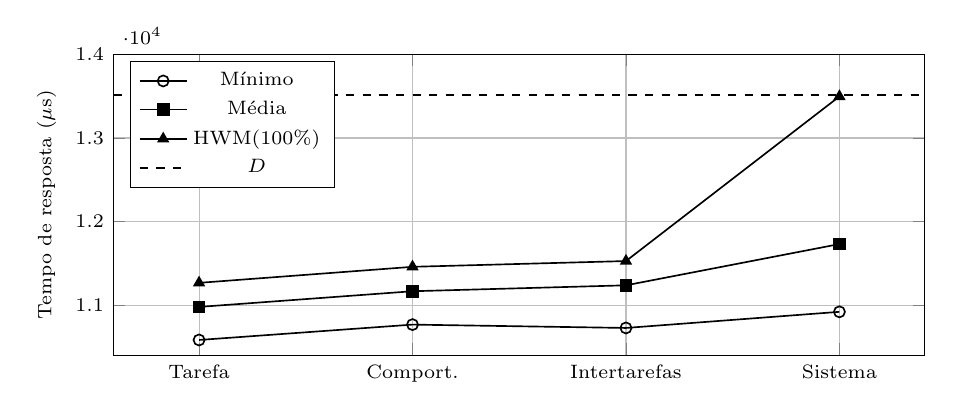
\begin{tikzpicture}
\begin{axis}[width=0.98\columnwidth,height=5.4cm,xmin=0.6,xmax=4.4,ymin=10400,ymax=14000,
  xtick={1,2,3,4},xticklabels={Tarefa,Comport.,Intertarefas,Sistema},
  ylabel={Tempo de resposta ($\mu$s)},grid=major,
  tick label style={font=\scriptsize},label style={font=\scriptsize},
  legend style={font=\scriptsize,at={(0.02,0.98)},anchor=north west}]
\addplot[mark=o,semithick] coordinates {(1,10582)(2,10766)(3,10726)(4,10919)};
\addplot[mark=square*,semithick] coordinates {(1,10977.7)(2,11165.6)(3,11236.5)(4,11730.5)};
\addplot[mark=triangle*,semithick] coordinates {(1,11266)(2,11458)(3,11527)(4,13498)};
\addplot[dashed,semithick,domain=0.6:4.4,samples=2] {13519};
\legend{Mínimo,Média,HWM(100\%),$D$}
\end{axis}
\end{tikzpicture}
\caption{Mínimo, média e HWM por etapa ($N = 1\,000$) e o deadline fixo $D$.}
\end{figure}

\subsection{Leitura}
A mesma tarefa, com a mesma lógica, apresenta HWM crescente com o escopo: 11266 $\mu$s (etapa 1), 11458 $\mu$s (+192 $\mu$s, etapa 2), 11527 $\mu$s (+261 $\mu$s, etapa 3) e 13498 $\mu$s (+2232 $\mu$s, etapa 4). A média sobe pouco (de 10977,7 a 11730,5 $\mu$s), mas o HWM sobe quase 20\%: a concorrência afeta mais a cauda que o centro da distribuição. Medir só a tarefa isolada daria a impressão de um sistema com HWM de 11266 $\mu$s, quando o sistema completo chega a 13498 $\mu$s.

Na etapa 1, o HWM da construção da árvore foi de 7919 $\mu$s, o dos códigos, 1644 $\mu$s, o da codificação, 874 $\mu$s, e o da decodificação, 831 $\mu$s. A construção da árvore responde por cerca de 70\% do HWM total.

O maior HWM da etapa 4 ($N = 1\,000$) fica a apenas 21 $\mu$s de $D$. Uma rodada com a etapa 4 e o watchdog de tarefas ligado foi descartada: os \emph{backtraces} impressos durante a medição elevaram o HWM a 38060 $\mu$s, com 872 perdas. Isso indica que a tarefa \texttt{IDLE0} deixou de rodar no core 0: a carga, a Huffman periódica e a Huffman por evento, juntas, saturaram o core.

\section{Experimento B: convergência do HWM}
\subsection{Descrição}
O objetivo é saber com quantas amostras o HWM parece estabilizar, se há saltos tardios e se, com poucas amostras, o sistema pareceria mais rápido do que é. A atividade executada foi rodar o cenário completo da etapa 4 (sensor, Huffman periódica medida, evento e carga) com 10\,000 ativações da Huffman periódica, em vez das 1\,000 das demais rodadas. O firmware registra o tempo de resposta de cada ativação e, depois da medição, imprime o HWM acumulado após 10, 20, 100, 1\,000 e 10\,000 amostras. A rodada B usou o firmware dedicado ao experimento; as outras duas rodadas de 10\,000 ativações vieram do experimento D, que faz a mesma medição. Todas usaram a mesma configuração (texto de 1\,000 caracteres, semente 12345, watchdog de tarefas desligado). Cada rodada leva cerca de 7 minutos.

\subsection{Resultados}
A Tabela IV e a Figura 2 mostram o HWM acumulado nas três rodadas.

\begin{table}[!t]
\centering
\caption{HWM acumulado ($\mu$s) na etapa 4, em função do número de amostras.}
\small
\setlength{\tabcolsep}{4pt}
\begin{tabular}{lrrrrr}
\toprule
Rodada & 10 & 20 & 100 & 1\,000 & 10\,000 \\
\midrule
B & 12484 & 12484 & 13032 & 13464 & 13464 \\
D, rodada 1 & 12478 & 12478 & 12993 & 13292 & 13490 \\
D, rodada 2 & 12492 & 12492 & 13030 & 13319 & 13459 \\
\bottomrule
\end{tabular}
\end{table}

\begin{figure}[!t]
\centering
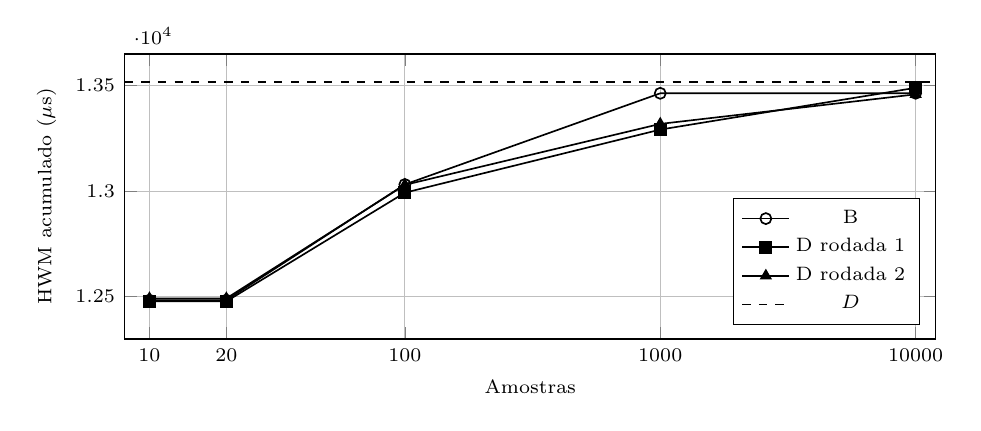
\begin{tikzpicture}
\begin{axis}[width=0.98\columnwidth,height=5.2cm,xmode=log,xmin=8,xmax=12000,ymin=12300,ymax=13650,
  xtick={10,20,100,1000,10000},xticklabels={10,20,100,1000,10000},xminorticks=false,
  xlabel={Amostras},ylabel={HWM acumulado ($\mu$s)},grid=major,
  tick label style={font=\scriptsize},label style={font=\scriptsize},
  legend style={font=\scriptsize,at={(0.98,0.05)},anchor=south east}]
\addplot[mark=o,semithick] coordinates {(10,12484)(20,12484)(100,13032)(1000,13464)(10000,13464)};
\addplot[mark=square*,semithick] coordinates {(10,12478)(20,12478)(100,12993)(1000,13292)(10000,13490)};
\addplot[mark=triangle*,semithick] coordinates {(10,12492)(20,12492)(100,13030)(1000,13319)(10000,13459)};
\addplot[dashed,semithick,domain=8:12000,samples=2] {13519};
\legend{B,D rodada 1,D rodada 2,$D$}
\end{axis}
\end{tikzpicture}
\caption{Convergência do HWM acumulado na etapa 4.}
\end{figure}

\emph{Com 10 ou 20 amostras, o sistema pareceria mais rápido do que é.} O HWM com 10 e 20 amostras ficou entre 12478 e 12492 $\mu$s, ou seja, cerca de 1 ms (7\%) abaixo do HWM com 10\,000 amostras. Com 100 amostras, o HWM já estava a 3\% a 4\% do valor final, e com 1\,000, a no máximo 1,5\%.

\emph{Houve saltos tardios.} Entre 1\,000 e 10\,000 amostras, o HWM subiu 198 $\mu$s na rodada 1 do experimento D e 140 $\mu$s na rodada 2; na rodada B, ele ficou em 13464 $\mu$s. Portanto, com 10\,000 amostras, o HWM não estabilizou em duas de três rodadas, e o valor final variou de 13459 a 13490 $\mu$s entre rodadas. O HWM é um limite inferior do WCRT, e deve ser acompanhado de margem.

\section{Experimento C: margem de segurança}
\subsection{Descrição}
O objetivo é saber em que etapa uma margem fixa deixa de ser suficiente e se uma margem fixa é adequada quando a variabilidade muda. Este experimento não exigiu nova rodada: é um cálculo sobre os HWMs já medidos nas etapas 1 a 4. Cada margem (10\%, 25\% e 50\%) é aplicada ao HWM da etapa 1 (11266 $\mu$s), multiplicando-o por 1,10, 1,25 e 1,50. O valor resultante é comparado com o maior HWM entre as rodadas de cada etapa (11266, 11458, 11527 e 13498 $\mu$s). A folga é a margem menos o HWM da etapa; quando ela é negativa, a margem não cobre aquela etapa.

\subsection{Resultados}
A Tabela V mostra a folga (positiva) ou a falta (negativa) de cada margem.

\begin{table}[!t]
\centering
\caption{Margem sobre o HWM da etapa 1 e folga ($\mu$s) em relação ao HWM de cada etapa.}
\small
\setlength{\tabcolsep}{3pt}
\begin{tabular}{lrrrrr}
\toprule
Margem & Valor & Etapa 1 & Etapa 2 & Etapa 3 & Etapa 4 \\
\midrule
10\% & 12393 & +1127 & +935 & +866 & $-1105$ \\
25\% & 14083 & +2817 & +2625 & +2556 & +585 \\
50\% & 16899 & +5633 & +5441 & +5372 & +3401 \\
\bottomrule
\end{tabular}
\end{table}

A margem de 10\% é suficiente até a etapa 3 e deixa de ser na etapa 4: o HWM do sistema (13498 $\mu$s) exige 19,8\% sobre o HWM da etapa 1. A margem de 25\% cobre as quatro etapas, mas a folga na etapa 4, de 585 $\mu$s, é cerca de 4\% do valor da margem. A de 50\% cobre com sobra, e torna o $D$ pouco útil para detectar perdas.

Uma margem fixa só é adequada se a variabilidade se mantém. Aqui ela muda: a diferença entre o HWM e o mínimo passa de 684 $\mu$s na etapa 1 para 2579 $\mu$s na etapa 4, ou seja, cerca de 3,8 vezes maior. Isso lembra o exemplo da aula, em que a variação passa de 12--14 ms para 10--16 ms (de 2 a 6 ms, o triplo): a margem escolhida com a tarefa isolada não acompanha a variabilidade do sistema.

\section{Experimento D: perdas de deadline e (m,k)-firme sob diferentes deadlines}
\subsection{Descrição e procedimento}
O objetivo é medir como o percentual de deadlines cumpridos, o \emph{skip factor} e o (m,k)-firme mudam quando só o deadline varia, e encontrar o menor $D$ que satisfaz um (m,k) exigido na etapa 4. A atividade executada foi rodar o cenário da etapa 4 com $N = 10\,000$, em duas rodadas, e deixar o firmware calcular as perdas para cada $D$ depois da medição.

O experimento usa a etapa 4 com $N = 10\,000$, em duas rodadas. Os tempos de resposta ficam em memória e, depois da medição, o firmware recalcula as perdas para três valores de $D$: 11266 $\mu$s (HWM da etapa 1, sem margem), 12393 $\mu$s (margem de 10\%) e 13519 $\mu$s (o $D$ do trabalho). Também varre $D$ de 11000 a 14000 $\mu$s, em passos de 100 $\mu$s, e calcula a pior janela para $k = 20$. Como $D$ é só um limite sobre as mesmas medições, as diferenças entre valores de $D$ vêm exclusivamente do critério.

\subsection{Resultados}
A Tabela VI mostra os resultados para os três valores de $D$, nas duas rodadas, e a Figura 3 mostra o percentual no prazo na varredura.

\begin{table*}[!t]
\centering
\caption{Etapa 4 ($N = 10\,000$): resultados por $D$, na rodada 1 / rodada 2.}
\small
\setlength{\tabcolsep}{4pt}
\begin{tabular}{rlrrrrrrr}
\toprule
$D$ ($\mu$s) & Origem & \% no prazo & Perdas & $S$ & Maior rajada & (m,k) $k{=}10$ & (m,k) $k{=}20$ & (m,k) $k{=}50$ \\
\midrule
11266 & HWM(100\%) da etapa 1 & 15,09 / 15,03 & 8491 / 8497 & 1 & 39 / 38 & (0,10) & (0,20) & (1,50) \\
12393 & Margem de 10\% & 89,97 / 89,99 & 1003 / 1001 & 1 & 2 / 2 & (7,10) & (16,20) / (15,20) & (42,50) / (41,50) \\
13519 & $D$ do trabalho & 100 / 100 & 0 / 0 & n/a & 0 / 0 & (10,10) & (20,20) & (50,50) \\
\bottomrule
\end{tabular}
\end{table*}

\begin{figure}[!t]
\centering
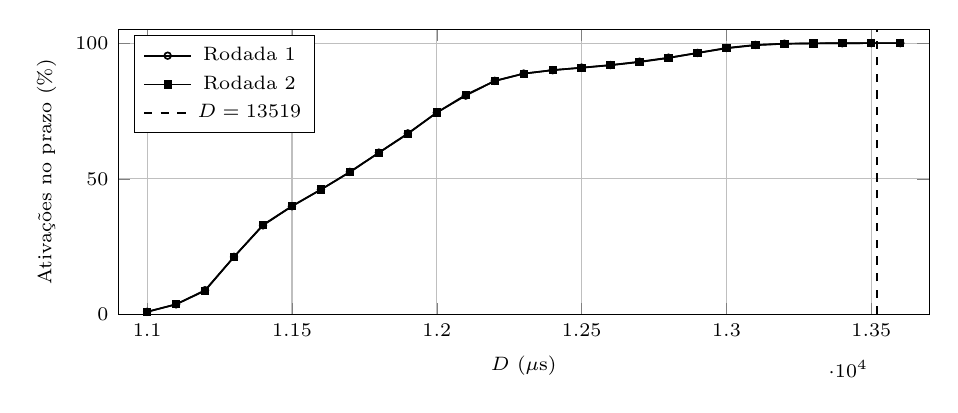
\begin{tikzpicture}
\begin{axis}[width=0.98\columnwidth,height=5.2cm,xmin=10900,xmax=13700,ymin=0,ymax=105,
  xlabel={$D$ ($\mu$s)},ylabel={Ativações no prazo (\%)},grid=major,
  tick label style={font=\scriptsize},label style={font=\scriptsize},
  legend style={font=\scriptsize,at={(0.02,0.98)},anchor=north west}]
\addplot[mark=o,mark size=1.2pt,semithick] coordinates {(11000,0.98)(11100,3.75)(11200,8.95)(11300,21.24)(11400,32.84)(11500,39.88)(11600,46.05)(11700,52.56)(11800,59.65)(11900,66.74)(12000,74.40)(12100,80.67)(12200,86.10)(12300,88.78)(12400,90.03)(12500,90.97)(12600,91.93)(12700,93.16)(12800,94.64)(12900,96.40)(13000,98.23)(13100,99.35)(13200,99.79)(13300,99.92)(13400,99.96)(13500,100)(13600,100)};
\addplot[mark=square*,mark size=1.2pt,semithick] coordinates {(11000,0.99)(11100,3.74)(11200,8.76)(11300,21.25)(11400,33.02)(11500,39.95)(11600,46.03)(11700,52.44)(11800,59.59)(11900,66.58)(12000,74.41)(12100,80.96)(12200,86.04)(12300,88.75)(12400,90.07)(12500,90.92)(12600,91.86)(12700,93.03)(12800,94.52)(12900,96.36)(13000,98.10)(13100,99.24)(13200,99.77)(13300,99.90)(13400,99.97)(13500,100)(13600,100)};
\addplot[dashed,semithick] coordinates {(13519,0)(13519,105)};
\legend{Rodada 1,Rodada 2,$D = 13519$}
\end{axis}
\end{tikzpicture}
\caption{Percentual de ativações no prazo em função de $D$ (etapa 4, $N = 10\,000$).}
\end{figure}

Com $D = 11266\ \mu$s, apenas 15\% das ativações cumprem o prazo, porque a média do sistema (11733 $\mu$s) já está acima desse valor. Com $D = 12393\ \mu$s, cerca de 90\% cumprem, e as perdas aparecem isoladas ou em pares. Com $D = 13519\ \mu$s, nenhuma ativação perde o prazo nas duas rodadas, com folga de 29 e 60 $\mu$s sobre o HWM.

\subsection{Menor $D$ para um (m,k) exigido}
A Tabela VII mostra o menor $D$ da varredura (resolução de 100 $\mu$s) que satisfaz cada (m,20)-firme exigido.

\begin{table}[!t]
\centering
\caption{Menor $D$ ($\mu$s) que satisfaz o (m,20)-firme, rodada 1 / rodada 2.}
\small
\setlength{\tabcolsep}{3pt}
\begin{tabular}{lrrr}
\toprule
(m,k) exigido & Menor $D$ & \% no prazo & Folga até 13519 \\
\midrule
(16,20) & 12400 / 12400 & 90,03 / 90,07 & 1119 / 1119 \\
(17,20) & 12600 / 12500 & 91,93 / 90,92 & 919 / 1019 \\
(18,20) & 13100 / 13100 & 99,35 / 99,24 & 419 / 419 \\
(19,20) & 13300 / 13200 & 99,92 / 99,77 & 219 / 319 \\
(20,20) & 13500 / 13500 & 100 / 100 & 19 / 19 \\
\bottomrule
\end{tabular}
\end{table}

Reduzir $D$ em cerca de 3\% (de 13519 para 13100 $\mu$s) ainda mantém (18,20)-firme, mas com 65 a 76 perdas em 10\,000 ativações. Exigir (19,20) permite um $D$ de 219 a 319 $\mu$s menor que o do trabalho, e exigir (20,20), isto é, nenhuma perda, leva praticamente ao próprio HWM (13500 $\mu$s contra o HWM de 13459 a 13490 $\mu$s).

\subsection{Perdas isoladas ou em rajada}
Com $D = 11266\ \mu$s, as perdas formam rajadas de até 39 ativações consecutivas, o que equivale a cerca de 1,6 s sem cumprir prazo (cerca de 42 ms por ciclo). Com $D = 12393\ \mu$s, as perdas são isoladas ou em pares (maior rajada 2). O \emph{skip factor} é $S = 1$ em todos os $D$ com perdas, porque sempre há duas perdas em ativações consecutivas; por isso ele é pouco informativo aqui, e a distribuição das rajadas e o (m,k) descrevem melhor o comportamento.

Em um sistema com inércia física, o que importa é o tempo entre perdas consecutivas, não só o percentual: um atuador tolera uma ou duas perdas isoladas, que a inércia do sistema absorve, mas não 39 seguidas. Dois $D$ com o mesmo percentual de perdas podem ter comportamentos opostos, um com perdas espaçadas e outro com uma única rajada longa. No $D$ de 12393 $\mu$s, a rodada 1 mostra perdas a cada 8 ativações no início da execução (ativações 7, 30, 38, 46, 54, 62, 70, 78, 86, 94); a causa desse padrão não foi investigada.

\section{(m,k)-firme: significado e limites}
Uma tarefa é (m,k)-firme se cumpre pelo menos $m$ deadlines em qualquer janela de $k$ ativações consecutivas. O (m,k) medido é calculado pela janela deslizante: $m = k - p_{\max}$. Ele transforma uma série de perdas em um critério testável: por exemplo, a etapa 4 com $D = 12393\ \mu$s exibe (7,10), (16,20) e (42,50) na rodada 1 e (7,10), (15,20) e (41,50) na rodada 2. Nas etapas 1 a 3, e na etapa 4 com $D = 13519\ \mu$s, o (m,k) é $(k,k)$.

O (m,k) obtido descreve o comportamento observado nas medições; ele não é uma garantia formal. Os limites aparecem nos próprios dados:
\begin{itemize}
\item \emph{Variação entre rodadas.} Com o mesmo $D$ e a mesma carga, o (m,20) variou de (16,20) para (15,20) entre duas rodadas.
\item \emph{Dependência do $D$.} O mesmo sistema exibe (0,20) com $D = 11266\ \mu$s e (20,20) com $D = 13519\ \mu$s.
\item \emph{HWM ainda crescente.} Como o HWM subiu depois de 1\,000 amostras em duas de três rodadas, uma rodada mais longa ou diferente pode ter perdas que as medidas não registraram, inclusive com $D = 13519\ \mu$s.
\item \emph{Janelas e entrada.} O resultado vale para as sementes, as cargas e os valores de $k$ avaliados, em um número limitado de rodadas.
\end{itemize}

\section{Ameaças à validade}
\begin{itemize}
\item \emph{Plataforma:} a ESP32 com FreeRTOS não é um sistema de propósito geral. O tick de 10 ms faz com que o despertar das tarefas só ocorra em múltiplos de 10 ms, o que explica parte da variação do instante de liberação.
\item \emph{Estados ocultos:} cache de instruções e de flash, estado da SRAM e aquecimento da placa não foram controlados.
\item \emph{Interrupções do sistema:} o evento é um \emph{timer} do ESP-IDF executado em uma tarefa de alta prioridade, não uma interrupção de hardware. Isso adiciona latência ao disparo.
\item \emph{Instrumentação:} \texttt{clock\_gettime} e a cópia do buffer entram no tempo medido. Os períodos com \texttt{vTaskDelay} passam a ser contados a partir do fim da ativação anterior.
\item \emph{Watchdog desligado:} o watchdog de tarefas ficou desligado nas rodadas de sistema. Como o programa termina sozinho, não houve travamento, mas a proteção contra travamento foi removida.
\item \emph{Cenários de estresse:} a carga é só de CPU, no core 0, junto com as Huffman. Rede e outros periféricos não foram usados como estresse, e o pior caso de concorrência de hardware pode ser diferente.
\item \emph{Aplicação de $D$:} no experimento D, os valores de $D$ são aplicados depois da medição, o que mostra o efeito do critério, não o comportamento de um sistema configurado com outro deadline.
\item \emph{Número de rodadas:} três rodadas por etapa com $N = 1\,000$ e três com $N = 10\,000$ não bastam para uma estatística de convergência.
\end{itemize}

\section{Conclusão}
Com a mesma lógica de codificação, o HWM cresceu com o escopo de teste: de 11266 $\mu$s (tarefa) para 13498 $\mu$s (sistema), cerca de 20\%, com a média subindo bem menos. O aumento não vem de novos caminhos lógicos, mas da concorrência com outras tarefas, da carga e do mutex, que o teste da tarefa isolada não alcança. Mesmo no sistema, o HWM continuou subindo depois de 1\,000 amostras em duas de três rodadas, então o HWM observado deve ser tratado como uma estimativa otimista do WCRT.

A margem de 10\% sobre o HWM da etapa 1 é insuficiente para o sistema; a de 25\% cobre, com folga de 585 $\mu$s. O deadline $D = 13519\ \mu$s foi cumprido em todas as ativações de todas as etapas, mas com folga de apenas 21 a 60 $\mu$s sobre o HWM da etapa 4.

Quando o WCRT não é alcançável, o modelo (m,k)-firme descreve o comportamento observado em uma faixa de $D$: com $D = 12393\ \mu$s, o sistema exibe (16,20) e (15,20) nas duas rodadas, e exigir (18,20) permite um $D$ 3\% menor que o adotado. Esse (m,k) é uma descrição do que foi medido, não uma garantia, e varia com o $D$, com a rodada e com a carga.

O código-fonte, os registros de cada etapa e as saídas do monitor estão em \url{https://github.com/Thifjj/Sistemas-em-tempo-real} (diretório \texttt{atividade\_m3}).

\begin{thebibliography}{1}
\bibitem{enunciado} Professores M. Douglas C. A. e F. Viel, ``Atividade M3: estimativa de WCRT com medições,'' enunciado, Sistemas em Tempo Real, UNIVALI, 2026.
\end{thebibliography}

\end{document}
